\documentclass{article}
\usepackage{epsfig, latexsym}

\begin{document}

\newcommand{\bs}{\backslash}

\title{
\Large{CMPEN 271 -- Fall 2009}\\
\normalsize{Exam 2}\\
\makebox[4in][l]{Name:} 
PSU ID:}
\date{}

\maketitle{}


\begin{enumerate}
\item {\bf (2 pts.)} Assuming a word size of 5 bits, interpret 10101 as a 2's complement number.

\begin{tabular}{p{0.6in} p{0.6in} p{0.6in} p{0.6in} l}
a) -24 & b) -12 & c) -6 & d) -2 & e) None of the above.
\end{tabular}

\item {\bf (2 pts.)} Assuming a word size of 4 bits, determine the 2's complement
representation of -7.

\begin{tabular}{p{0.6in} p{0.6in} p{0.6in} p{0.6in} l}
a) 1011 & b) 1101 & c) 1100 & d) 1001 & e) None of the above.
\end{tabular}


\underline{For questions 3,4 assume that espresso has generated the following output.}
\begin{verbatim}
.i 3
.o 2
.ilb A B C
.ob F G
.p 3
1-1 10
01- 11
-01 01
.e
\end{verbatim}

\item{\bf (1 pt.)}  Which product term is shared.
\begin{description}
\item{a) } AC
\item{b) } A'B
\item{c) } B'C
\item{d) } F and G
\end{description}


\item{\bf (1 pt.)}  Which of the following could be equal to G(A,B,C)?
\begin{description}
\item{a) } G(A,B,C) = $\Sigma$m(1,2,3,5)
\item{b) } A'B'C + A'BC + A'BC' + AB'C
\item{c) } A'B + B'C
\item{d) } G(A,B,C) = $\prod$M(0,4,6,7)
\item{e) } All of the above
\end{description}

\item {\bf (2 pts.)} How many 1:2 decoders does it take to build a 3:8 decoder?

\begin{tabular}{p{0.6in} p{0.6in} p{0.6in} p{0.6in} l}
a) 3 & b) 7 & c) 15 & d) 31 & e) None of the above.
\end{tabular}

\item {\bf (1 pt.)} If the delay through a single 2:1 mux is 1 unit of time,
then what is the delay through a 16:1 mux built from 2:1 muxes?

\begin{tabular}{p{0.6in} p{0.6in} p{0.6in} p{0.6in} l}
a) 2 & b) 4 & c) 8 & d) 15 & e) None of the above.
\end{tabular}

\item {\bf (2 pts.)} How many inputs do the AND gates in a 8:1 mux have?

\begin{tabular}{p{0.6in} p{0.6in} p{0.6in} p{0.6in} l}
a) 2 & b) 4 & c) 8 & d) 16 & e) None of the above.
\end{tabular}

\item {\bf (1 pt.)} How many 4:1 muxes are needed to construct a 8-bit 4:1 mux?

\begin{tabular}{p{0.6in} p{0.6in} p{0.6in} p{0.6in} l}
a) 4 & b) 8 & c) 12 & d) 32 & e) None of the above.
\end{tabular}

Questions 9-11 concern the construction of a bit-slice of a comparator.  
The questions will ask you to complete the entries in the truth table 
below denoted by $a$, $b$, and $c$.

\begin{tabular}{l|l|l|l|l||l|l|l}
$G_{in}$ & $L_{in}$ & $E_{in}$ & $x$ & $y$ & $G_{out}$ & $L_{out}$ & $E_{out}$ \\ \hline
    0    &    0     &     1    &  0  &  0  &   $a$     &           &  \\ \hline
    0    &    1     &     0    &  1  &  0  &           &   $b$     &  \\ \hline
    1    &    0     &     1    &  1  &  0  &           &           &  $c$    \\
\end{tabular}

\item {\bf (1 pt.)}What is the value of $a$?

\begin{tabular}{p{0.6in} p{0.6in} p{0.6in}}
a) 0 & b) 1 & c) x 
\end{tabular}

\item {\bf (1 pt.)}What is the value of $b$?

\begin{tabular}{p{0.6in} p{0.6in} p{0.6in}}
a) 0 & b) 1 & c) x 
\end{tabular}

\item {\bf (1 pt.)}What is the value of $c$?

\begin{tabular}{p{0.6in} p{0.6in} p{0.6in}}
a) 0 & b) 1 & c) x 
\end{tabular} \\

\underline{ Use the following figure for questions 12,13.}

\includegraphics{./Fig2/compare2}

\item {\bf (1 pt.)} Which of $G,L,E$ below must be connected to the
sel input of the mux to realize: \verb+if (X >=  Y) then Z = X else Z = Y;+

\begin{tabular}{p{0.6in} p{0.6in} l}
a) G & b) L & c) E 
\end{tabular}


\item {\bf (2 pt.)} Which of $X,Y$ must be connected to the $y_0$ input
of the mux?

\begin{tabular}{p{0.6in} l}
a) X & b) Y  
\end{tabular}

\begin{tabular}{llll}
\begin{tabular}{c||c}
D & Q+   \\ \hline
0 & 0 \\ \hline
1 & 1 \\
\end{tabular}
&
\begin{tabular}{c||c}
T & Q+   \\ \hline
0 & Q \\ \hline
1 & Q' \\
\end{tabular}
&
\begin{tabular}{c|c||c}
S & R & Q+   \\ \hline
0 & 0 & Q \\ \hline
0 & 1 & 0 \\ \hline
1 & 0 & 1 \\ \hline
1 & 1 & x \\
\end{tabular}
&
\begin{tabular}{c|c||c}
J & K & Q+   \\ \hline
0 & 0 & Q \\ \hline
0 & 1 & 0 \\ \hline
1 & 0 & 1 \\ \hline
1 & 1 & Q' \\
\end{tabular}
\end{tabular}

\underline{For questions 14-19 use the following figure.}

\scalebox{0.7}{\includegraphics{./Fig2/ExTim3}}

\item {\bf (2 pts.)} What is the value of Q1 at time 25

\begin{tabular}{p{0.75in}p{0.75in}p{1.75in}}
a) 0 & b) 1 & c) toggling \\
\end{tabular}

\item {\bf (2 pts.)} What is the value of Q1 at time 35

\begin{tabular}{p{0.75in}p{0.75in}p{1.75in}}
a) 0 & b) 1 & c) toggling \\
\end{tabular}

\item {\bf (2 pts.)} What is the value of Q1 at time 65

\begin{tabular}{p{0.75in}p{0.75in}p{1.75in}}
a) 0 & b) 1 & c) toggling \\
\end{tabular}

\item {\bf (2 pts.)} What is the value of Q2 at time 25

\begin{tabular}{p{0.75in}p{0.75in}p{1.75in}}
a) 0 & b) 1 & c) toggling \\
\end{tabular}

\item {\bf (2 pts.)} What is the value of Q2 at time 35

\begin{tabular}{p{0.75in}p{0.75in}p{1.75in}}
a) 0 & b) 1 & c) toggling \\
\end{tabular}

\item {\bf (2 pts.)} What is the value of Q2 at time 65

\begin{tabular}{p{0.75in}p{0.75in}p{1.75in}}
a) 0 & b) 1 & c) toggling \\
\end{tabular}

\pagebreak

\item {\bf (2 pts.)} Which line of pseudo-code best characterizes
the following piece of hardware.

\scalebox{0.7}{\includegraphics{./Fig2/conditional}}

\begin{description}
\item{a) } \verb^if (X < Y) then Z = X+3 else Z = Y+3;^
\item{b) } \verb^if (X < Y) then Z = Y+3 else Z = X+3;^
\item{c) } \verb^if (X > Y) then Z = X+3 else Z = Y+3;^
\item{d) } \verb^if (X > Y) then Z = Y+3 else Z = X+3;^
\item{e) } None of the above
\end{description}

In problems 21,22 you are designing a circuit which multiplies
a 4-bit binary number by (decimal) 10.

\item {\bf (1 pt.)} How many bits wide does the result have to be?

\begin{tabular}{p{0.6in} p{0.6in} p{0.6in} p{0.6in} l}
a) 4 & b) 5 & c) 6 & d) 8 & e) None of the above. \\
\end{tabular}

\item {\bf (1 pt.)} What is the fewest number of adders required?

\begin{tabular}{p{0.6in} p{0.6in} p{0.6in} p{0.6in} l}
a) 1 & b) 2 & c) 3 & d) 9 &  e) 10 \\
\end{tabular}


\pagebreak
You have a digital design which calls for a circuit which performs the 
following task (written as a C if/then statement).  You have decided on 
the architecture.  Its your job to design to complete the truth table
for the the glue-logic box (only an arbitrary portion of the complete 
truth table is shown).  I would recommend drawing a number line 
and putting the values of L6, L12, and L18 on it.  

\begin{verbatim}
if      (sum < 6)  z = sum
else if (sum < 12) z = sum-6
else if (sum < 18) z = sum-12
else               z = sum-18
\end{verbatim}

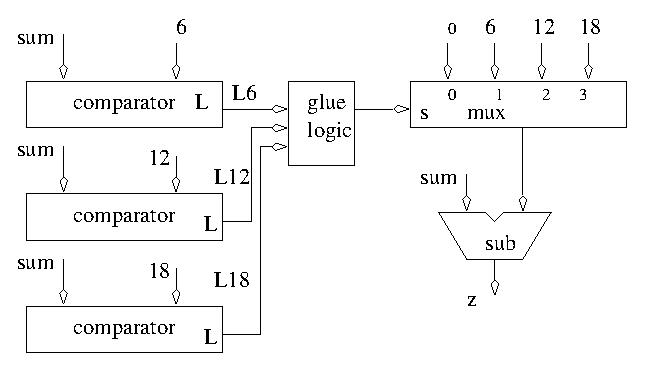
\includegraphics{./Fig2/if6}

\vspace{0.25in}

\begin{tabular}{l|l|l||l}
L6 & L12 & L18 & select \\ \hline
0  & 0   & 0   &   a   \\ \hline
0  & 1   & 1   &   b   \\ \hline
1  & 0   & 1   &   c   \\ 
\end{tabular}

\vspace{0.25in}

\item {\bf (2 pts.)}What is the (decimal) value of a in the truth table?

\begin{tabular}{p{0.6in} p{0.6in} p{0.6in} p{0.6in} l}
a) 0 & b) 1 & c) 2 & d) 3 & e) x  
\end{tabular}

\item {\bf (2 pts.)}What is the (decimal) value of b in the truth table?

\begin{tabular}{p{0.6in} p{0.6in} p{0.6in} p{0.6in} l}
a) 0 & b) 1 & c) 2 & d) 3 & e) x  
\end{tabular}

\item {\bf (2 pts.)}What is the (decimal) value of c in the truth table?

\begin{tabular}{p{0.6in} p{0.6in} p{0.6in} p{0.6in} l}
a) 0 & b) 1 & c) 2 & d) 3 & e) x  
\end{tabular}


\end{enumerate}
\end{document}
